\documentclass[varwidth=true,varwidth=\maxdimen]{standalone}
\usepackage{lmodern}
% (2) specify encoding
\usepackage[T1]{fontenc}

% (3) load symbol definitions
\usepackage{textcomp}
\usepackage{tikz}
\usepackage{ifthen}
\usetikzlibrary{arrows,positioning}

% Load tikz library in file "tikzlibraryBES.code.tex"
\tikzset{
   % House
   hcnode/.style={circle,draw,fill=blue!30, minimum size=30},
   hclink/.style={text=blue!30,fill=blue!30},
   hclabel/.style={text width= 2cm, align=center},
   % hypercube label pics
   pics/hclabels/.style args={#1/#2/#3}{
   code={
 
      % for convience using 0 to 7
      % \node[hclabel] (h10) at (0,0)
      \foreach \c [count=\x from 0] in {{0\textunderscore0},{0\textunderscore1},{0\textunderscore2},{0\textunderscore3},{1\textunderscore1},{1\textunderscore0}, {1\textunderscore3},{1\textunderscore2}} 
        \ifthenelse{\x = #1}
            {}
            {
                % loop through list of colored nodes
                \foreach\n/\co in {#3}
                \ifthenelse{\x = \n}
                {\node[text=\co!60] at (0,-0.5*\x) {#2 $ \rightarrow $ \c};}
                {\node at (0,-0.5*\x) {#2 $ \rightarrow $ \c};}
                ;
            }
        ;
    }},
   pics/hclabels/.default=0/0\textunderscore0/35,
   % hypercube
   pics/hypercube/.style args={#1/#2/#3}{
   code={
      % Define house parameters
      \newcommand\wallheight{#1}  % 0.65
      \newcommand\roofoverhang{#2}  % 0.15
      \newcommand\roofangle{#3}  % 35

      % Calculate some dependent sizes
      \pgfmathsetmacro\lengthroof{0.5/cos(\roofangle)+\roofoverhang}

      % draw profile of house
      % \draw[line width=1pt] (-0.5,\wallheight) -- (-0.5,0) --  (0.5,0) -- (0.5,\wallheight) -- ++(-\roofangle:\roofoverhang) -- ++(180-\roofangle:\lengthroof) -- ++(180+\roofangle:\lengthroof) -- cycle;
      \node[hcnode] at (0, 0) (00) {0\textunderscore0};
      \node[hcnode] at (3, 0) (01) {0\textunderscore1};
      \node[hcnode] at (0, -3) (02) {0\textunderscore2};
      \node[hcnode] at (3, -3) (03) {0\textunderscore3};
      
      \node[hcnode] at (10, 0) (11) {1\textunderscore1};
      \node[hcnode] at (13, 0) (10) {1\textunderscore0};
      \node[hcnode] at (10, -3) (13) {1\textunderscore3};
      \node[hcnode] at (13, -3) (12) {1\textunderscore2};
      
      % Arrows last
      % Draw blue links
      \path[draw,blue!30] (00) -- (01) -- (03) -- (02) -- (00);
      \path[draw,blue!30] (11) -- (10) -- (12) -- (13) -- (11);
      % inner links
      \draw [-,blue!30] (01) to [out=30,in=150] (11);
      \draw [-,blue!30] (03) to [out=-30,in=-150] (13);
      % outer links
      \draw [-,blue!30] (00) to [out=30,in=150] (10);
      \draw [-,blue!30] (02) to [out=-30,in=-150] (12);
      % Draw green links
      
      % Draw Red links
    }},
    pics/hypercube/.default=0.65/0.15/35
}

\begin{document}
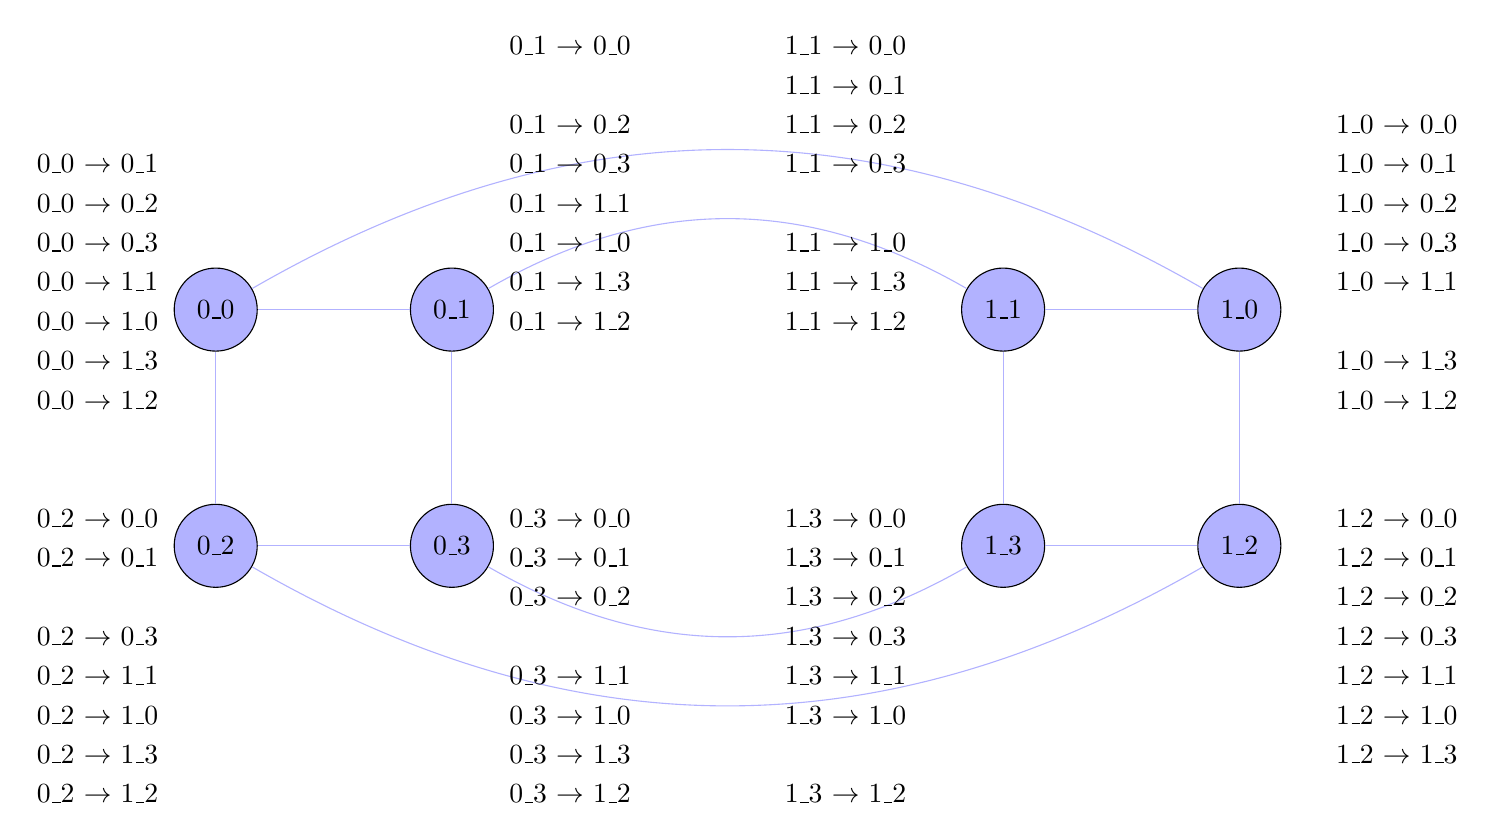
\begin{tikzpicture}
 \path (+1.5,-0.85) pic[scale=1.0] {hypercube};
  % Labels for Node 0 
 \path (0,1.5) pic[scale=1.0] {hclabels=0/0\textunderscore0/{0/black}};
  % Labels for Node 2
 \path (0,-3.5) pic[scale=1.0] {hclabels=2/0\textunderscore2/{2/black}};
  % Labels for Node 1
  \path (6,2.5) pic[scale=1.0] {hclabels=1/0\textunderscore1/{1/black}};
  % Labels for Node 3
  \path (6,-3.5) pic[scale=1.0] {hclabels=3/0\textunderscore3/{3/black}};
  
% Labels for Node 0 
 \path (16.5,1.5) pic[scale=1.0] {hclabels=5/1\textunderscore0/{5/black}};
  % Labels for Node 2
 \path (16.5,-3.5) pic[scale=1.0] {hclabels=7/1\textunderscore2/{7/black}};
  % Labels for Node 1
  \path (9.5,2.5) pic[scale=1.0] {hclabels=4/1\textunderscore1/{4/black}};
  % Labels for Node 3
  \path (9.5,-3.5) pic[scale=1.0] {hclabels=6/1\textunderscore3/{6/black}};
\end{tikzpicture}
% 
% \newline
% \begin{tikzpicture}
% \path (0,0) pic[scale=1.0] {hclabels=0/0\textunderscore0/{1/red,4/green}};
%  \path (+1.5,-0.85) pic[scale=1.0] {hypercube};
% \end{tikzpicture}
% \begin{tikzpicture}

% \path (+1.5,-0.85) pic[scale=1.0] {hypercube};

% \end{tikzpicture}
\end{document}